\ExplSyntaxOn
\NewDocumentCommand{\blankpages}{m}
 {
  \clearpage
  \prg_replicate:nn { #1 } { \mbox{}\thispagestyle{plain}\clearpage }
 }
\ExplSyntaxOff

% Chapter 2

\chapter{Line of research and contributions} % Main chapter title

\label{Chapter2} % For referencing the chapter elsewhere, use \ref{Chapter1} 

\section{Improved wind forecasting using kernel regression for circular variables}

\subsection{Introduction}
The first part of this thesis is focused on exploring how classic non-linear regression methodologies can be used to improve the output of numerical weather models. Multivariate linear regression is a classic method for modelling the relationship between a scalar output variable and one or more input variables. This method serves in many cases as the baseline method when comparing new approaches to do regression, so we decided to start our research by exploring the most fundamental techniques.

\medskip

The challenge in this case is to perform regression on the NWP wind speed variable using observed data. Wind is a weather phenomenon that is highly dependent on topography. Wind is normally represented using vectors, where the module provides the speed and the angle is the direction of the wind. Weather models decompose the wind speed variable into its Cartesian components to simplify its representation. The problem with this approach is that performing operations such as regression is not straight forward because of the relationship and dependence between both components.

\medskip

For this study, we use the Global Forecasting System (GFS) NWP model and Aviation Routine Weather Reports (METARs) from three airports in northern Spain, Vitoria-Gasteiz, Bilbao and San Sebastian-Donostia. The GFS model represents data using a regular grid which covers the whole world, with a spatial resolution of approximately 50 km and a temporal resolution of 3 hours. This model is operated by the National Oceanographic and Atmospheric Administration (NOAA) and the global dataset for the latest 15 years is made publicly available. METARS are high quality meteorological reports drafted in most of the civil airports in the world. These reports are made available every 30 minutes and describe variables such as wind, temperature, visibility and cloud coverage at the airport's runway. METARS are encoded as text messages and distributed worldwide so flight control groups and pilots can plan take off and landing procedures.

\medskip

For each of the three airports we selected the NWP grid points closest to the observation points, creating a temporal series that contains both the modeled and observed values for different weather parameters. We compare different linear and non-linear regression methodologies using different combinations of NWP variables in the input and using the observed wind speed as the output variable.

\medskip

The reason for choosing wind speed as the output is because this variable is highly affected by the local topography surrounding the airports. Airports are normally located in open spaces with constant and wind patterns. These three airports in northern Spain are placed in a mountainous region near the Atlantic coast and have very specific wind regimes which are highly affected by the local topography. The resolution of the NWP model used in this study is in the order of 75 km, which means that these three airports are modeled in contiguous grid cells. The work is focused on studying the potential of observed wind speed data to correct the NWP values for specific locations.

\subsection{Research contribution}

Non-parametric regression is a category of regression analysis in which the predictor does not take a predetermined form but is built each time from the data. Non-parametric regression requires larger sample sizes than regression based on parametric models because the data must supply the model structure as well as the model estimates. This work demonstrates a technique using non-parametric regression for improving wind speed prediction by clustering wind speed data around specific directional components. This regression is performed dynamically, selecting historical data with similar characteristics. The level of similarity and the relative weights for each element in the regression is controlled using different shapes of kernels.

\medskip

\begin{figure}[h]
 \centerline{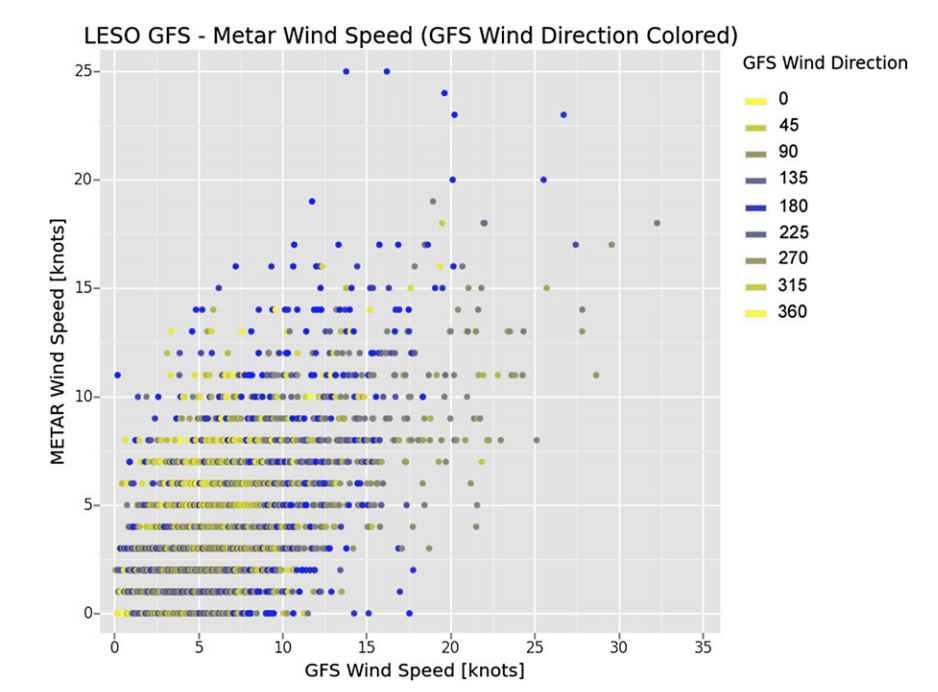
\includegraphics[width=10cm]{paper1.png}}\caption{Relationship between GFS and METAR wind speed values from San Sebastian. GFS wind direction is represented using a color scale, with colors around yellow showing northerly winds and colors around blue representing southerly winds.}\label{paper1}
\end{figure}

For example, Figure \ref{paper1} contains a representation of the relationship between the observed and forecasted the wind values generated for one of the studied airports. In this case, wind direction is used in a cyclic kernel to dynamically weight the contribution of each input data point in the regression.

\medskip

This work introduces the concept of cyclic kernel which provides a way of clustering elements using a circular variable. We demonstrate how circular kernels can  successfully assimilate
directional data into a regression model. This concept can also extend and improve other circular or temporal variables and can be used to extract seasonal or daily patterns from data.

\subsection{Publication: A Method for Wind Speed Forecasting in Airports Based on Nonparametric Regression}

This work was published in the "Weather and Forecasting" journal, which is a scientific publication from the American Meteorological Society. This publication covers articles on weather forecasting and analysis techniques, forecast verification studies, and case studies useful to forecasters. It was first submitted to the journal in March 2014 and was finally published in December 2014 after a major revision process that required work on improving the statistical method used to validate the methodology.

\blankpages{10}

%----------------------------------------------------------------------------------------

\section{Circular regression trees}

\subsection{Introduction}

Most of the current regression machine learning algorithms are focused on modelling the relationships between linear variables. Circular variables have a different nature to linear variables, so traditional methodologies are not able to represent their content thoroughly, leading to suboptimal results in most cases.

\medskip

Continuing with the study of methodologies for modelling circular variables, we decided to focus on regression trees for this new research study. Regression trees and tree based ensemble methods, such as bagging or Random Forest, are a versatile, computationally efficient and accurate method for performing regression. Building upon the pioneering concept of circular regression tree \citep{lund2002tree}, we decided to explore alternative and more efficient methods for introducing circular variables in regression trees.

\medskip

Traditionally, circular variables have been used in regression trees using two approaches. The first one ignores the circular nature of a variable treating it as linear variable. The problem with this approach is that 0 and 360 degrees are represented at each end of the variable range, when in reality they are the same value. The second approach is to decompose a circular variable into its Cartesian components and use them as separate variables in a tree. Both of these approaches introduce constrains and limit the performance of regression trees. With the first approach, trees cannot perform splits that cross the origin, and in the second case splits performed on the Cartesian components independently lead to an excessive and unnatural partition of the space defined by circular variables having a negative impact in the accuracy of the resulting models. 

\medskip

For this work we use a similar dataset to the one introduced in the previous section about non-linear kernel regression. We choose to forecast the observed speed of the wind at 5 different locations in Europe. Data from airport METARS of Berlin Tegel, London Heathrow, Barcelona El Prat, Paris Charles de Gaulle and Milano Malpensa are used to train the different tree models and to analyse the results. Similarly to the previous work we extract the time series data from the GFS model for the closest grid cells to each of these airports. The tree models are trained using three-hourly data for the years 2011, 2012 and 2013, providing approximately 8760 samples per airport.


\subsection{Research contribution}
The key idea behind circular trees is that circular variables can be naturally integrated in regression trees by considering splits that cross the origin [0-360] point in the search space. The original implementation of circular trees performs splits on non-contiguous regions of the variable space leading to excessive fragmentation of the dataset. The improvement proposed in our work restricts the search space to contiguous regions of the variable space leading to an improvement in computation performance and accuracy of the results. Figure \ref{paper2} contains a representation of the splits performed by our circular tree for a dataset that contains one circular and one linear variable. The splits generated by this tree define contiguous regions in the space.

\medskip

In this work we introduce a new methodology that restricts the search space of each partition in a tree generating contiguous partitions. This constraint added to the initial idea of circular regression trees in Lund's work \citep{lund2002tree} has the implication of generating more simple partitions which improve the accuracy of the tree model and is more efficient to train. Although the search space for optimal splits at each node of the tree is more limited than the original version, which allows non-contiguous splits, the overall error of the tree results to be lower as the depth of the tree increases in our case. In this work we found that even if non-contiguous splits provide good results at the top part of a tree, these partitions tend to degenerate as the partition process evolves resulting in trees with poor performance.

\medskip

\begin{figure}[h]
 \centerline{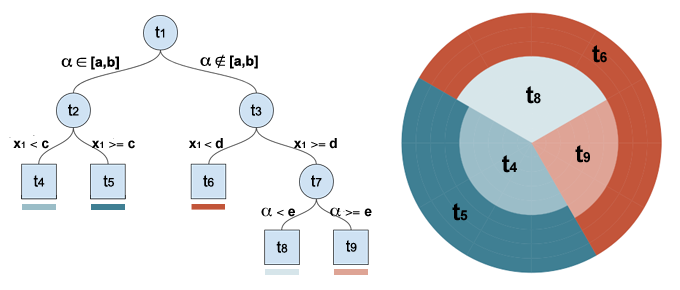
\includegraphics[width=10cm]{paper2.png}}\caption{Example of the proposed circular regression tree and a representation of how the space is divided in contiguous regions.}\label{paper2}
\end{figure}

The software developed in this work is presented in the form of a self-contained Python library. This library implements a general version of regression tree which can be used with both linear and circular variables in the input and output. Also, there is an option to perform non-contiguous partitions, as in the original proposal by Lund \citep{lund2002tree} and contiguous as in the metodology that we propose.  The library also offers a command line interface that allows users to train and test different regression tree models and download datasets for any airport in the world. These tools have been designed so users can create their own forecasts experimenting and exploring the differences between models, input variables and airports. The scripts and libraries are written in a simple way so users can read the code to understand what the program is doing and also modify or extend its functionalities. AeroCirTree comes with a GNU GPLv3 licence so anyone can use, modify and share this program for any purpose.

\subsection{Publication: A system for airport weather forecasting based on circular regression trees}

In March 2017 it was submitted to the "Environmental Modelling \& Software", a peer-reviewed scientific journal which publishes work involving modelling and software within the Environmental Science domain. The work was finally published in February 2018, after a major revision process that required extra work to demonstrate the benefit of our circular methodology in comparison to other linear trees alternatives.

\blankpages{10}

%----------------------------------------------------------------------------------------

\section{Convolutional neural networks for image regression}

\subsection{Introduction}
During the time of working on the circular regression tree, deep learning techniques where presented to the research community demonstrating unprecedented results in many different domains. Although, as far as we knew, there were not applications in the meteorological domain in the literature we decided to learn and apply these techniques to weather forecasting problems. Convolutional neural networks, used mainly on image classification tasks, seemed a good candidate to model NWP gridded data.

\medskip

Up until this point in our research, we extracted data from the closest NWP grid point to the desired observed dataset resulting in a time series. Convolutional Neural Networks (CNN) offer the possibility of treating a whole image as the input to a model and the neural network can learn to detect the regions of the image that are most correlated with the output. This is a major change on how we were doing research compared to our two previous works. CNNs do not require to know the location of the individual grid points as an input, they can treat the whole weather grids (images) as their only input avoiding the need of extracting temporal series beforehand.

\medskip

CNNs are mainly used to perform classification and extraction of spatial information in images, building from fine grained details into higher level structures. In this work we explored the use of CNNs to classify the event of precipitation (rain/dry) at different cities in Europe. 

\medskip

CNN require large data sets to be trained. For this work we used a different dataset called ERA-Interim \citep{dee2011era} which contains data since the year 1979, with a temporal resolution of 3 hours. This dataset is publicly available from the European Centre for Medium-Range Weather Forecasts (ECMWF). This dataset is generated using a numerical weather model which simulates the state of the atmosphere for the whole planet, with a spatial resolution of approximately 80 km. The output is presented in the form of regular numerical grids and there is a large number of physical parameters available, representing variables such as temperature, wind speed and relative vorticity.

\medskip

For determining the event of rain at the different locations we use Aviation Routine Weather Reports (METARs) similarly to our previous works. We consider 5 main airports located in different cities across Europe and a period of 5 years (2012-2017). The airports are: Helsinki-Vanta, Amsterdam-Schiphol, Dublin, Rome-Fiumicino and Vienna.

\medskip

We extract an extended area over Europe from ERA-Interim, creating a 3 hourly series of images composed by 3 bands, corresponding to the geopotential height \textbf{z} at the 1000, 700 and 500 pressure levels of the atmosphere. This parameter represents the height in the atmosphere at which a certain pressure value is reached. These levels correspond typically to 100, 3000 and 5500 metres above the mean sea level respectively.

\subsection{Research contribution}

In this work we experimented adding the temporal dimension to the CNN network. The temporal dimension is added to these networks by adding a fourth axis to the convolutional kernels (latitude, longitude, height, time). Using the collection of geopotential fields as input and the precipitation conditions for the different locations as output, the CNN networks are trained to predict the rain conditions at each point. Although we are not giving the coordinates of the different locations within the pressure field, the network succeeds at finding the relationship between both. This work demonstrates therefore that CNNs can be used to interpret the output of NWP to generate local forecasts automatically.

\medskip

Also as part of this work we used a technique called Class Activation Mapping (CAM) \citep{zhou2016learning} to introspect inside the CNN models and visually assess the regions of the input space that have more influence in the output. The use of CAM is represented in Figure \ref{paper3} using a heat-map to represent the relative weight of each pixel in the network. It can be seen how the network learns to give more weight to the pixels surrounding the region even when this parameter is not known to the network.

\medskip

Also in this work, 3D convolutions are proven to be able to naturally incorporate the temporal component of the data into neural networks, resulting in a significant improvement in the accuracy of the results when compared to a similar network trained with individual frames.

\begin{figure}[h]
 \centerline{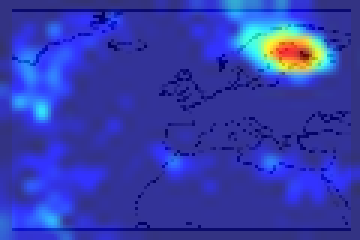
\includegraphics[width=5cm]{paper3_2.png}\\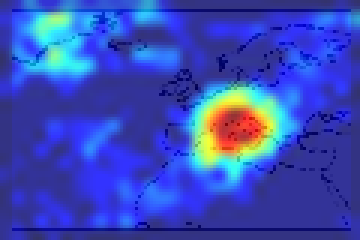
\includegraphics[width=5cm]{paper3_1.png}}\caption{Example of the resulting Class Activation Maps for an ERA-Interim CNN trained using the observed precipitation at Helsinki-Vantaa airport, EFHK, (left) and Rome Fiumicino airport, LIRF, (right). Coastlines have been overlaid as a reference for readers.}\label{paper3}
\end{figure}


\subsection{Publication: Automating weather forecasts based on convolutional networks}

This work was accepted for the "Deep Structured Prediction" workshop celebrated as part of the 2017 ICML conference in Sydney. The work was presented in July 2017 at the workshop and I received positive feedback on the techniques and a few people asked about the nature and availability of the dataset.

\blankpages{10}

%----------------------------------------------------------------------------------------

\section{Convolutional encoder-decoders for image to image regression}

\subsection{Introduction}
The work presented at the 2017 ICML conference led and motivated us to continue researching the field and applications of Convolutional Neural Networks (CNN). Being aware of the demonstrated capacity that CNNs have to extract the spatial structure from input images, we decided to explore the possibilities that these techniques had in the field of meteorology.

\medskip

For this new research work we focused on studying NWP parameterisations. There are physical processes in the atmosphere that cannot be represented by NWP regardless of its resolution. For these physical processes that cannot be directly resolved, NWP uses approximate models, which are known as parameterisations.

\medskip

To perform the experiments in this work, we use the ERA-Interim global climate reanalysis dataset produced by the European Centre for Medium-Range Weather Forecasts (ECMWF). ERA-Interim makes available a large number of parameters, from which we choose geopotential height and total precipitation. We crop an extended area over Europe and extracted the selected parameters over the 1980-2016 period with a temporal resolution of 6 hours, resulting in dataset with more than 50,000 samples. 


\subsection{Research contribution}

Autoencoders \citep{hinton2006reducing} are generic neural networks that recreate the input by performing a dimensionality reduction and subsequent expansion of the input space. This technique allows learning compressed representations of the data in an unsupervised manner. Convolutional autoencoders combine CNNs with autoencoders to efficiently learn compressed representations of images. A latter evolution of convolutional autoencoders demonstrates that similar networks offer an efficient way of performing image segmentation by training the model with samples of segmented images. Figure \ref{paper4} contains a representation of the transformations performed by an encoder-decoder network to the geopotential field transforming it into a precipitation field for the same region.

\medskip

We consider three different state-of-the-art convolutional encoder-decoder networks in the field of image segmentation: VGG-16 \citep{long2015fully}, Segnet \citep{badrinarayanan2017segnet} and U-net \citep{ronneberger2015u}. These networks are modified to perform image regression tasks instead of segmentation by changing the loss function to MAE and tested with the task of predicting precipitation.

\medskip

This work demonstrates that convolutional encoder-decoder neural networks can be used, as an alternative to parameterisations, to learn complex atmospheric processes using basic NWP fields as input. As far as we know, this is the first attempt to provide an end-to-end automated learning approach to derive new parameterisations from basic NWP fields using deep convolutional encoder-decoder networks. This work also demonstrates how popular deep learning networks in the field of image segmentation can be adapted to interpret and derive new weather parameters.

\medskip

\begin{figure}[h]
 \centerline{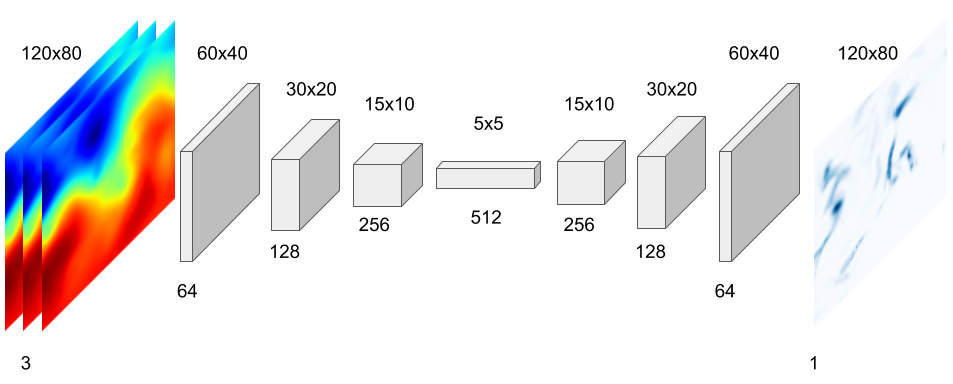
\includegraphics[width=10cm]{paper4.png}}\caption{Representation of the transformations performed by the encoder-decoder network to the geopotential height field and its transformation into a field representing the total precipitation field for the same region.}\label{paper4}
\end{figure}

\subsection{Publication: Learning parameterisations with encoder-decoder convolutional neural networks}

This work was first submitted in June 2018 to the "Monthly Weather Review", which is a peer-reviewed scientific journal published by the American Meteorological Society. It covers research related to analysis and prediction of observed and modeled circulations of the atmosphere, including technique development, data assimilation, model validation, and relevant case studies.

\medskip

The editor of the journal wrote us a few weeks after our submission expressing his interest in the techniques presented in our work and proposing major changes in the contents of the manuscript. The main concern was about the language and references presented in our work, which where not suitable to the public of this journal. 

\medskip

The paper was rewritten providing an introduction to machine learning and CNNs in the context of weather forecasting and NWP parameterisations. It was submitted again in October 2018.

\blankpages{10}